% %File: anonymous-submission-latex-2024.tex
% \documentclass[letterpaper]{article} % DO NOT CHANGE THIS
% \usepackage[submission]{aaai24}  % DO NOT CHANGE THIS
% \usepackage{times}  % DO NOT CHANGE THIS
% \usepackage{helvet}  % DO NOT CHANGE THIS
% \usepackage{courier}  % DO NOT CHANGE THIS
% \usepackage[hyphens]{url}  % DO NOT CHANGE THIS
% \usepackage{graphicx} % DO NOT CHANGE THIS
% \urlstyle{rm} % DO NOT CHANGE THIS
% \def\UrlFont{\rm}  % DO NOT CHANGE THIS
% \usepackage{natbib}  % DO NOT CHANGE THIS AND DO NOT ADD ANY OPTIONS TO IT
% \usepackage{caption} % DO NOT CHANGE THIS AND DO NOT ADD ANY OPTIONS TO IT
% \frenchspacing  % DO NOT CHANGE THIS
% \setlength{\pdfpagewidth}{8.5in} % DO NOT CHANGE THIS
% \setlength{\pdfpageheight}{11in} % DO NOT CHANGE THIS
% %
% % These are recommended to typeset algorithms but not required. See the subsubsection on algorithms. Remove them if you don't have algorithms in your paper.
% \usepackage{algorithm}
% \usepackage{algorithmic}


% \usepackage{booktabs}
% \usepackage{amsmath}
% \usepackage[table]{xcolor}
% \usepackage{amssymb}

% % added by ns
% \usepackage{multirow}
% \usepackage{threeparttable}

% %
% % These are are recommended to typeset listings but not required. See the subsubsection on listing. Remove this block if you don't have listings in your paper.
% \usepackage{newfloat}
% \usepackage{listings}
% \DeclareCaptionStyle{ruled}{labelfont=normalfont,labelsep=colon,strut=off} % DO NOT CHANGE THIS
% \lstset{%
% 	basicstyle={\footnotesize\ttfamily},% footnotesize acceptable for monospace
% 	numbers=left,numberstyle=\footnotesize,xleftmargin=2em,% show line numbers, remove this entire line if you don't want the numbers.
% 	aboveskip=0pt,belowskip=0pt,%
% 	showstringspaces=false,tabsize=2,breaklines=true}
% \floatstyle{ruled}
% \newfloat{listing}{tb}{lst}{}
% \floatname{listing}{Listing}
% %
% % Keep the \pdfinfo as shown here. There's no need
% % for you to add the /Title and /Author tags.
% \pdfinfo{
% /TemplateVersion (2024.1)
% }

% % DISALLOWED PACKAGES
% % \usepackage{authblk} -- This package is specifically forbidden
% % \usepackage{balance} -- This package is specifically forbidden
% % \usepackage{color (if used in text)
% % \usepackage{CJK} -- This package is specifically forbidden
% % \usepackage{float} -- This package is specifically forbidden
% % \usepackage{flushend} -- This package is specifically forbidden
% % \usepackage{fontenc} -- This package is specifically forbidden
% % \usepackage{fullpage} -- This package is specifically forbidden
% % \usepackage{geometry} -- This package is specifically forbidden
% % \usepackage{grffile} -- This package is specifically forbidden
% % \usepackage{hyperref} -- This package is specifically forbidden
% % \usepackage{navigator} -- This package is specifically forbidden
% % (or any other package that embeds links such as navigator or hyperref)
% % \indentfirst} -- This package is specifically forbidden
% % \layout} -- This package is specifically forbidden
% % \multicol} -- This package is specifically forbidden
% % \nameref} -- This package is specifically forbidden
% % \usepackage{savetrees} -- This package is specifically forbidden
% % \usepackage{setspace} -- This package is specifically forbidden
% % \usepackage{stfloats} -- This package is specifically forbidden
% % \usepackage{tabu} -- This package is specifically forbidden
% % \usepackage{titlesec} -- This package is specifically forbidden
% % \usepackage{tocbibind} -- This package is specifically forbidden
% % \usepackage{ulem} -- This package is specifically forbidden
% % \usepackage{wrapfig} -- This package is specifically forbidden
% % DISALLOWED COMMANDS
% % \nocopyright -- Your paper will not be published if you use this command
% % \addtolength -- This command may not be used
% % \balance -- This command may not be used
% % \baselinestretch -- Your paper will not be published if you use this command
% % \clearpage -- No page breaks of any kind may be used for the final version of your paper
% % \columnsep -- This command may not be used
% % \newpage -- No page breaks of any kind may be used for the final version of your paper
% % \pagebreak -- No page breaks of any kind may be used for the final version of your paperr
% % \pagestyle -- This command may not be used
% % \tiny -- This is not an acceptable font size.
% % \vspace{- -- No negative value may be used in proximity of a caption, figure, table, section, subsection, subsubsection, or reference
% % \vskip{- -- No negative value may be used to alter spacing above or below a caption, figure, table, section, subsection, subsubsection, or reference

% \setcounter{secnumdepth}{2} %May be changed to 1 or 2 if section numbers are desired.

% % The file aaai24.sty is the style file for AAAI Press
% % proceedings, working notes, and technical reports.
% %

% % Title

% % Your title must be in mixed case, not sentence case.
% % That means all verbs (including short verbs like be, is, using,and go),
% % nouns, adverbs, adjectives should be capitalized, including both words in hyphenated terms, while
% % articles, conjunctions, and prepositions are lower case unless they
% % directly follow a colon or long dash
% %\title{Mining Fine-Grained Image-Text Alignment in CLIP for Zero-Shot Captioning via Text-Only Training}
% \title{Supplementary Material for Mining Fine-Grained Image-Text Alignment for Zero-Shot Captioning via Text-Only Training}
% \author{
%     %Authors
%     % All authors must be in the same font size and format.
%     Written by AAAI Press Staff\textsuperscript{\rm 1}\thanks{With help from the AAAI Publications Committee.}\\
%     AAAI Style Contributions by Pater Patel Schneider,
%     Sunil Issar,\\ 
%     J. Scott Penberthy,
%     George Ferguson,
%     Hans Guesgen,
%     Francisco Cruz\equalcontrib,
%     Marc Pujol-Gonzalez\equalcontrib
% }
% \affiliations{
%     %Afiliations
%     \textsuperscript{\rm 1}Association for the Advancement of Artificial Intelligence\\
%     % If you have multiple authors and multiple affiliations
%     % use superscripts in text and roman font to identify them.
%     % For example,

%     % Sunil Issar\textsuperscript{\rm 2},
%     % J. Scott Penberthy\textsuperscript{\rm 3},
%     % George Ferguson\textsuperscript{\rm 4},
%     % Hans Guesgen\textsuperscript{\rm 5}
%     % Note that the comma should be placed after the superscript

%     1900 Embarcadero Road, Suite 101\\
%     Palo Alto, California 94303-3310 USA\\
%     % email address must be in roman text type, not monospace or sans serif
%     proceedings-questions@aaai.org
% %
% % See more examples next
% }

% %Example, Single Author, ->> remove \iffalse,\fi and place them surrounding AAAI title to use it
% \iffalse
% \title{My Publication Title --- Single Author}
% \author {
%     Author Name
% }
% \affiliations{
%     Affiliation\\
%     Affiliation Line 2\\
%     name@example.com
% }
% \fi

% \iffalse
% %Example, Multiple Authors, ->> remove \iffalse,\fi and place them surrounding AAAI title to use it
% \title{My Publication Title --- Multiple Authors}
% \author {
%     % Authors
%     First Author Name\textsuperscript{\rm 1},
%     Second Author Name\textsuperscript{\rm 2},
%     Third Author Name\textsuperscript{\rm 1}
% }
% \affiliations {
%     % Affiliations
%     \textsuperscript{\rm 1}Affiliation 1\\
%     \textsuperscript{\rm 2}Affiliation 2\\
%     firstAuthor@affiliation1.com, secondAuthor@affilation2.com, thirdAuthor@affiliation1.com
% }
% \fi


% % REMOVE THIS: bibentry
% % This is only needed to show inline citations in the guidelines document. You should not need it and can safely delete it.
% \usepackage{bibentry}
% % END REMOVE bibentry

\setcounter{section}{0}

\begin{table*}[]
\centering
\small
\begin{tabular}{|l|c|c|c|c|c|}
\hline
& \# Trainable Parameter & \# Frozen Parameter & CC3M to MSCOCO(CIDEr) & MSCOCO(CIDEr) & Support Memory\\
\hline
CapDec & 181M & 0 & - & 0.918 & 0 \\
\hline
DeCap & 68M & 0 & 0.421 & 0.912 & 50,000 \\
\hline
Reproduced CapDec & 1.5M & 1.3B & 0.093 & 0.465 & 0 \\
\hline
Reproduced DeCap & 1.5M & 1.3B & 0.292 & 0.427 & 50,000 \\
\hline
MacCap & 5.7M & 1.3B &  0.525 & 0.687 & 0 \\
\hline
\end{tabular}
\label{tab:params}
\caption{The parameter size and captioning performance of baseline methods. We display zero-shot cross-domain and zero-shot in-domain captioning results from the main paper. The support memory is only used by DeCap, where 50,000 texts are used to construct a memory bank for inference.}
\end{table*}


\section{Detail of Baselines}
In this section, we provide a detailed explanation for the setting difference between our paper and previous methods DeCap\cite{DeCap}, CapDec\cite{CapDec}. The key difference is whether the language model or text decoder is trainable. DeCap and CapDec train the language model and achieve better performance in zero-shot in-domain captioning. However, we propose a more practical setting where the language model is frozen. The reason is that the large language model undergoes training through an auto-regression objective, thereby acquiring the capacity to proficiently execute a multitude of tasks, such as questing answering, translation, and automatic summarization. Training language model for a specific task leads to a degradation in other tasks, which is demonstrated in our zero-shot VQA experiments. Besides, the impressive performance of large language models comes with scale which makes finetuning language models computationally expensive. To provide a comprehensive picture, we collect the model parameters information in Table 1. We observe that the better performance of CapDec and DeCap in zero-shot in-domain captioning is achieved with more parameters, however, MacCap outperforms CapDec and DeCap in zero-shot cross-domain captioning with fewer parameters.

\section{Ablation Study on Hyperparameters}

\textbf{Noise Variance}
The noise injection is utilized to reduce the widely observed \textit{modality gap} phenomenon in CLIP embedding space. We show the impact of noise variance when generating the text-region feature mentioned in Section 4.2 of the main paper. The results are shown in Figure~\ref{figure:noise}. We observed the best performance is achieved at noise variance 0.016 which is the same as suggested in \cite{CapDec}. Noise variances smaller than 0.016 cause performance drop due to the \textit{modality gap} while noise variances larger than 0.016 introduce extensive semantic ambiguity in text reconstruction training.

\textbf{Number of Image Patches}
The sub-region feature aggregation in Section 4.3 of the main paper aims to extract the features of image subregions. We select image patches based on their attention scores as the patches with higher scores tend to contain more semantic information. We empirically study the number of selected patches, which indicates how much background information is introduced when generating captions. The results are shown in Figure~\ref{figure:seq}. We observe the best performance is achieved when the number of selected patches is the same as the number of noise-injected text-region features.


\begin{figure}[htb]
  \centering
  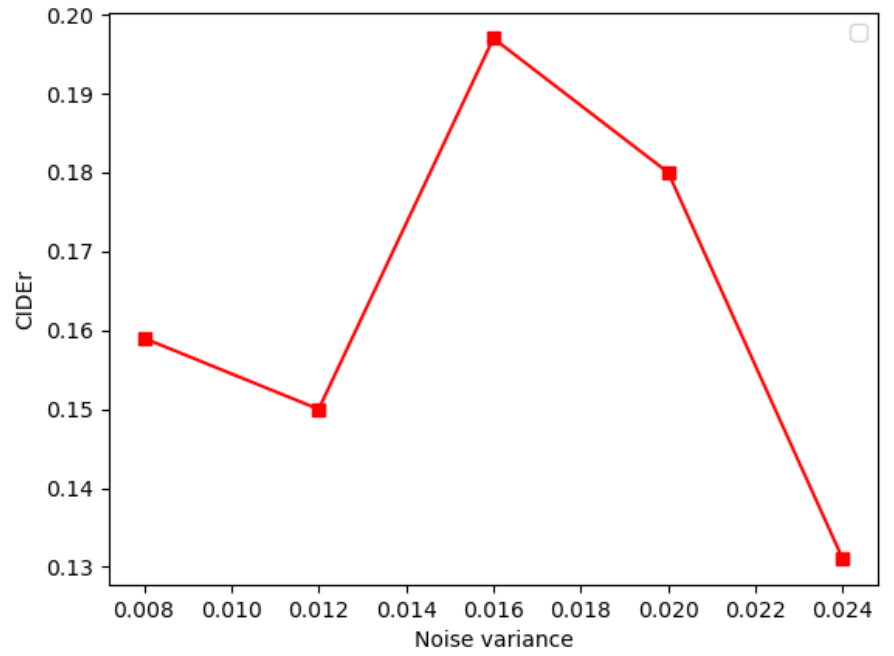
\includegraphics[width=0.4\textwidth]{AnonymousSubmission/LaTeX/asserts/supply_noise.png}
   \caption{\textbf{Performance of MacCap with different training noise.} The MacCap is trained in CC3M dataset and tested on Flickr30K datasets.}
    \label{figure:noise}
    \vspace{-0.2cm}
\end{figure}

\begin{figure}[bt]
  \centering
  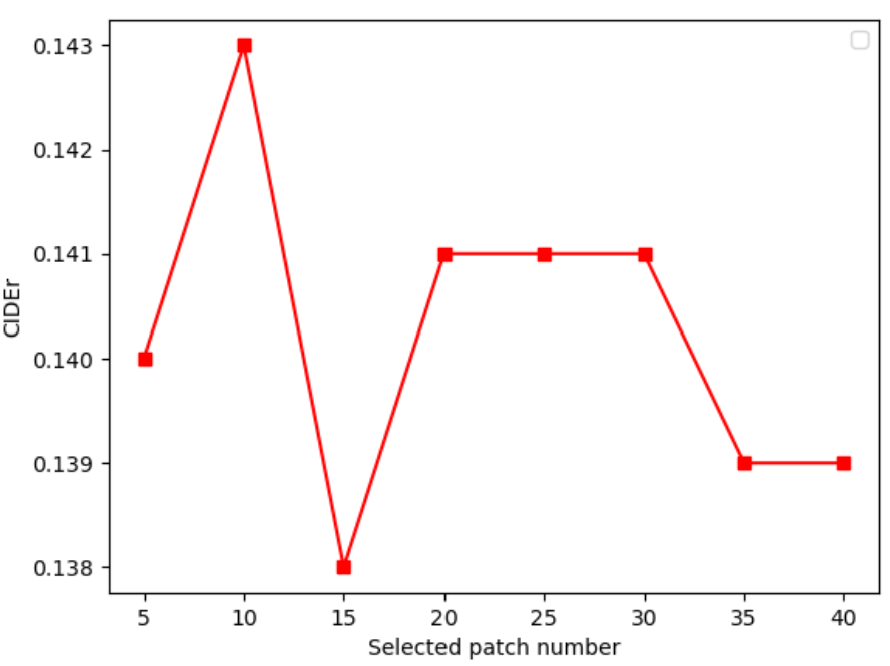
\includegraphics[width=0.4\textwidth]{AnonymousSubmission/LaTeX/asserts/seq_supply.png}
   \caption{\textbf{Performance of MacCap with different patch numbers in inference.} The MacCap is trained in CC3M dataset and tested on Flickr30K datasets. The length of the text region feature in text reconstruction training is set to 10.}
    \label{figure:seq}
    \vspace{-0.2cm}
\end{figure}


\section{Visualization of Image Sub-region}
In this section, we visualize the distribution of the global image embeddings, local image embeddings (i.e. the embeddings of image sub-region), and the text embeddings. We show the relation between image subregions and corresponding captions in Section 3.1 of the main paper, which reveals that subregion embeddings may have a higher similarity with the caption text embedding as they can be the specific image regions described by the accompanying caption. We visualize 5000 samples from the MSCOCO dataset with the dimensionality reduction method UMAP following \cite{MindGap}. The results are shown in Figure~\ref{figure:visulization}. We observe the distances between text embeddings are relatively small and all of the text embeddings are distributed near the (0, 0). Furthermore, there exists a modality gap between global image embedding and text embedding. The local image embeddings are distributed in the surrounding region of global image embeddings and are relatively closer to text embeddings than the global ones.

\begin{figure}[tb]
  \centering
  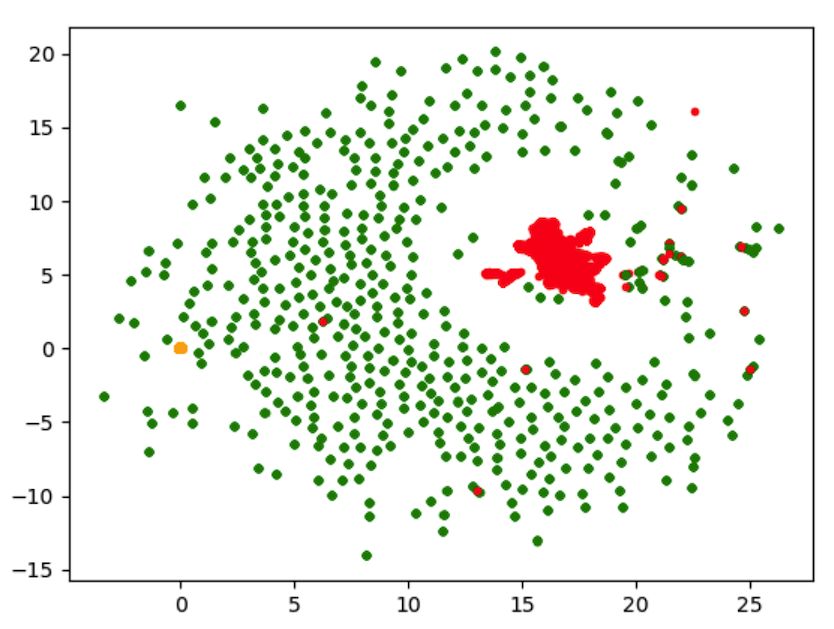
\includegraphics[width=0.4\textwidth]{AnonymousSubmission/LaTeX/asserts/nips_sup_vis.png}
   \caption{\textbf{Visualization of Embedding Distributions on MSCOCO.} The red points stand the global image embedding, each green point stand a local image embedding, and the yellow points near (0, 0) stand for the text embedding.}
    \label{figure:visulization}
    \vspace{-0.2cm}
\end{figure}


% 标题瞎写的
\section{Details of Modality Gap Distribution Analysis} 
In this section, we provide implementation details of modality gap distribution experiments.

We have text modality representation $T^i \in \mathbb{R}^D$ and vision modality representation. To be noticed, for vision modality, we have two sets of representations: the global embedding representing the overall information and the patch embeddings representing the image subregions information. The global embedding is $I_c^i \in \mathbb{R}^D$, and the patch embedding is $I_p^i \in \mathbb{R}^{N \times D}$. Both global embedding and local embedding are obtained by CLIP. $D$ is the dimension of CLIP embedding and $N$ is the sequence length of CLIP. $i \in \{1, 2, ... , num\_samples\}$

For paired images and text descriptions, we evaluate the gap between text representation and both global and patch image representation. For each image-text pair, we compute $G^c_i = T^i - I_c^i$ and $G^p_i = repeat(T^i, N) - I_p^i$. $G^c_i \in \mathbb{R}^{D}$, $G^p_i \in \mathbb{R}^{N \times D}$.

We can check the overall distribution over all $D$ dimensions. In this case, we treat data in all dimensions equally. We compute the mean over all image-text pairs and draw the histogram of the data distribution. Thus we compute the mean of the gap distribution for global vision and language representation as $Avg_{(i, d)} (I_c^i[d])$, and the gap for local vision and language representation as $Avg_{(i, s, d)} (I_p^i[s][d])$. $s \in [N], d \in [D]$.



